% 1979 年第 8 题：圆内接矩形 CEDF（C 在上、E 在左上、D 在下、F 在右），过 D 的切线与 CE 的延长线交于 A、与 CF 的延长线交于 B；连 DE、DF，CD 为直径（虚线）。按源卷布局：A、D、B 共线且为圆的切线，A、E、C 共线，C、F、B 共线。
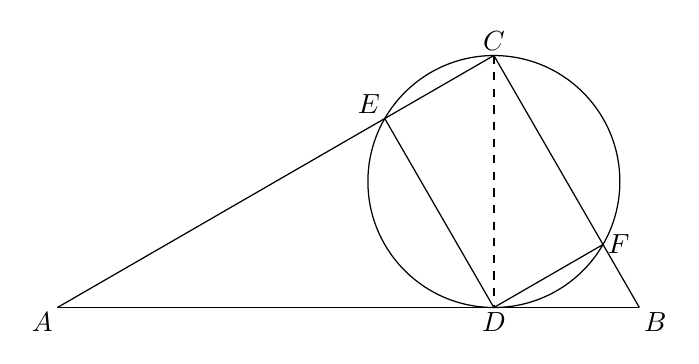
\begin{tikzpicture}[scale=1.6, line width=0.45pt,
  every node/.style={inner sep=1.5pt}]
  \coordinate (C) at (0,1);
  \coordinate (D) at (0,-1);
  \coordinate (E) at (-0.8660254,0.5);
  \coordinate (F) at (0.8660254,-0.5);
  \coordinate (A) at (-3.4641016,-1);
  \coordinate (B) at (1.1547005,-1);
  \draw (0,0) circle (1);
  \draw (A) -- (B);
  \draw (A) -- (C);
  \draw (C) -- (B);
  \draw (E) -- (D);
  \draw (D) -- (F);
  \draw[dashed] (C) -- (D);
  \node[anchor=south] at (C) {$C$};
  \node[anchor=south east] at (E) {$E$};
  \node[anchor=north] at (D) {$D$};
  \node[anchor=west] at (F) {$F$};
  \node[anchor=north east] at (A) {$A$};
  \node[anchor=north west] at (B) {$B$};
\end{tikzpicture}
